\section{Implementation}
\label{sec:implementation}

\subsection{Our System}

To understand the performance of our proposed method in common, real-world networks, we model our implementation with off-the-shelf smart home IoT devices. With our implementation based on the NVD, we narrow our focus to the $34$ devices that are both common and have corresponding vulnerabilities listed in the NVD. Live experiments are run on a network consisting of five of these devices: an Amazon Echo Dot, a Belkin WeMo, an HP Inkjet Envy printer, a Google Home Mini, and a Roku digital media player (see Figure \ref{fig:smart_home_network}).

\begin{figure}[t]
    \centering
    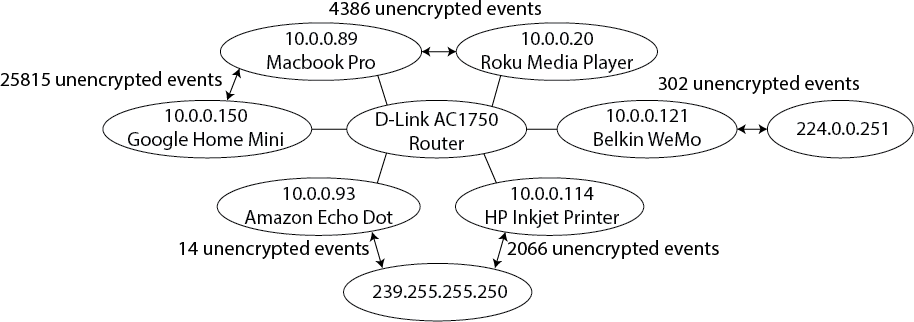
\includegraphics[width=0.5\textwidth]{smart_home_network.png}
    \caption{The smart-home network traffic graph corresponding to Figure \ref{fig:usage_over_time}.}
    \label{fig:smart_home_network}
\end{figure}

Our implementation is based on the CVE vulnerability database. Circuit construction is implemented using relevant CVEs in JSON format from NVD's database, with text processing using the Natural Language Toolkit (NLTK) \cite{bird2004nltk}. An example of the CVE processed as in Section \ref{subsubsec:input_output_extraction} is shown in Figure \ref{fig:processed_cve}. In this example, an \textit{input} (left of the arrow in the i/o field) is an action (DNS rebinding attack) that the attacker needs to take to leverage the corresponding vulnerability, in this case, CVE-2018-11314 (for access to root privileges or the configuration file). For each input, there is an \textit{output} (right of the arrow in the i/o field), which indicates the target that the attacker receives when once the input is applied to the vulnerability. A device may have multiple corresponding CVEs, a CVE may have multiple corresponding inputs, and an input may have multiple corresponding outputs. NetworkX \cite{hagberg2008exploring} and SNAP \cite{leskovec2016snap} are then used to build the attack circuit using these \textit{input/output} pairs and proceed with scoring.

\begin{figure}[t]
    \centering
    \begin{minipage}{0.5\textwidth}
    \begingroup\ttfamily\obeylines
    "Roku Media Player": [\{
    \ "description": "The External Control API in Roku and Roku TV products allow unauthorized access via a DNS Rebind attack.", 
    \ "id": "CVE-2018-11314", 
    \ "i/o": ["DNS Rebinding->this:Root 
    \ Priv", "DNS Rebinding->this:Config 
    \ File"]  \}]
    \endgroup
    \end{minipage}
    \caption{An example of a processed CVE data entry.}
    \label{fig:processed_cve}
\end{figure}

%An example of expoitability and impact attack circuits consisting of three devices (corresponding to the smart-home network shown in Figure \ref{fig:smart_home_network}) are shown in Figure \ref{fig:exploitability_circuit} and Figure \ref{fig:impact_circuit}. The edges of the graph are colored to represent expoitability capacity and impact weight, respectively.
% \begin{figure*}[t]
%     \centering
%     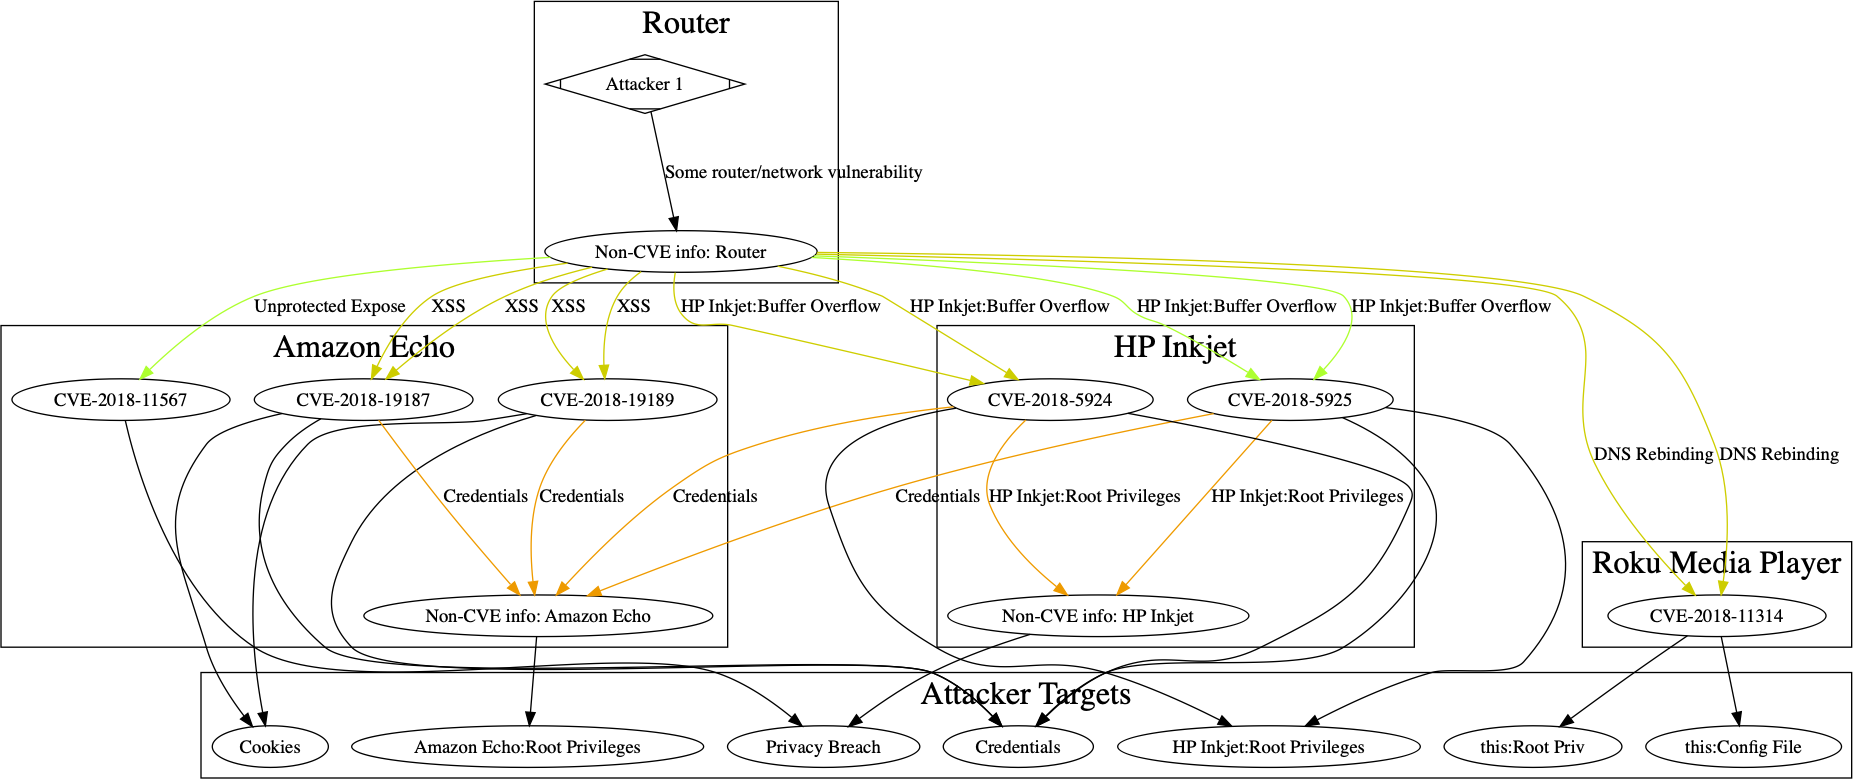
\includegraphics[width=\textwidth]{exploitability_circuit.png}
%     \caption{An example of an exploitability circuit.}
%     \label{fig:exploitability_circuit}
% \end{figure*}

% \begin{figure*}[t]
%     \centering
%     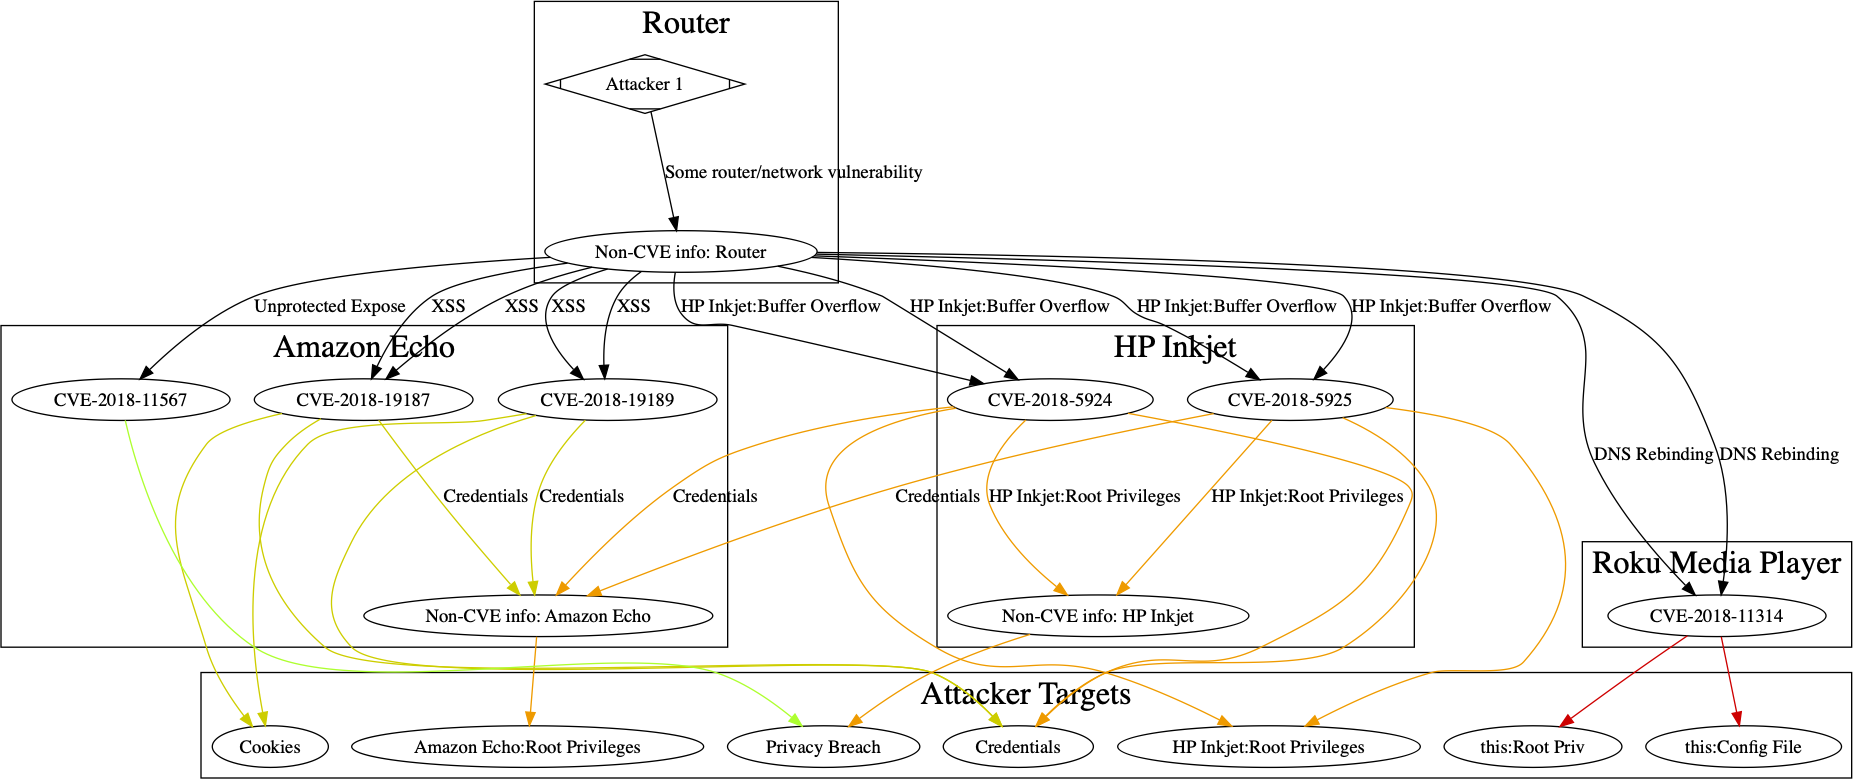
\includegraphics[width=\textwidth]{impact_circuit.png}
%     \caption{An example of an impact circuit.}
%     \label{fig:impact_circuit}
% \end{figure*}
\subsection{Our Scoring Method}

Let $EB_c \in [0,10]$ denote CVE $c$'s base exploitability score and $IB_c \in [0,10]$ denote CVE $c$'s base impact score. $EB_c, IB_c \in [0,10].$ We use impact and exploitability scoring guidelines set by the NVD in their CVSS v3 method\footnote{http://nvd.nist.gov/cvss.cfm}. The numerical possibilities for the CVSS metrics $AV$, $AC$, $PR$, $UI$, $I_{Conf}$, $I_{Integ}$, and $I_{Avail}$ can be found in Table 8.4 of the CVSS specification document. Scoring during the circuit construction phase is computed as shown in Equation \ref{eq:scoring_circuit_construction}. Numerical constants used are assigned based on empirical evaluation of the system. 

\begin{equation}
\begin{array}{ll@{}ll}
EB_c = 8.22 \times AV \times AC \times PR \times UI \\
ISC_{Base} = 1 - [(1-I_{Conf}) \times (1-I_{Integ}) \times (1-I_{Avail})] \\
\texttt{if Scope = unchanged}: IB_c = 6.42 \times ISC_{Base} \\
\texttt{else}: \ \ \  IB_c = 7.52 \times [ISC_{Base}-0.029] \\
\ \ \ \ \ \ \ \ \ \ \ \ \ \ \ \ \ \ \ \ - 3.25 \times [ISC_{Base}-0.02]^{15}
\end{array}
\label{eq:scoring_circuit_construction}
\end{equation}

Then let $EC_d$ denote device $d$'s compositional exploitability score and $IC_d$ denote device $d$'s compositional impact score. Let $c_i$ denote the set of CVEs with input to $c$ (where each device $d$ has a set of $c$ corresponding to each CVE), let $c_o$ denote the set of CVEs that $c$ has output to, and let $v_d$ denote a dampener variable (we used $v_d$ = 0.1). Scoring during the compositional phase is computed as shown in Equation \ref{eq:scoring_compositional}.

\begin{equation}
\begin{array}{ll@{}ll}
EC_d = {\displaystyle\sum_{c \in d}(EB_c+v_d\displaystyle\sum_{i\in c_i}{EB_i}}) \\
IC_d = {\displaystyle\sum_{c \in d}(IB_c+v_d\displaystyle\sum_{o\in c_o}{IB_o}}) \\
\end{array}
\label{eq:scoring_compositional}
\end{equation}

Next we compute the network traffic multipliers for impact and exploitability. Network traffic data is collected using Wireshark \cite{orebaugh2006wireshark} and is stored in .pcap format. This file is then converted to CSV for parsing. The data is specific to a network of $5$ IoT devices and a period of $4$ days. We use three metrics: device Network Uptime ($NU$), Encryption Scheme ($EN$), and whether IP sources or destinations were listed in an IP blacklist database\footnote{https://myip.ms/browse/blacklist} ($IP$). The weights we assigned to the different categories correspond to importance with respect to the score in consideration---for instance, when considering the exploitability score, the Network Uptime multiplier = $NU$ = \texttt{\{"always\_online": 1.6, "frequently\_online": 1.4, "rarely\_online": 1.07, "never\_online": 1\}}.

% \begin{figure}[t]
%     \centering
%     \begin{minipage}{0.5\textwidth}
%     \begingroup\ttfamily\obeylines
%     NU = \{
%     \ "always\_online": 1.6,
%     \ "frequently\_online": 1.4,
%     \ "rarely\_online": 1.07,
%     \ "never\_online": 1
%     \}
%     EN = \{
%     \ "not\_encrypted":1.5, 
%     \ "encrypted": 1
%     \}
%     IP = \{
%     \ "accessed": 5,
%     \ "not\_accessed": 1
%     \}
%     \endgroup
%     \end{minipage}
%     \caption{Category weights.}
%     \label{fig:category_weights}
% \end{figure}

The final exploitability and impact scores $E_d$, $I_d$ for a device $d$ are then calculated as shown in Equation \ref{eq:final_scores}, where $m_{E_i}$ is an exploitability-related network traffic multiplier (e.g. $NU$, $EN$), $m_{I_j}$ is an impact-related network traffic multiplier (e.g. $IP$), and $v_{n}$ is a normalizing variable (we use $v_{n_1}=v_{n_2}=100$). These scores are normalized to a range of $[0,1]$.
\begin{equation}
\begin{array}{ll@{}ll}
E_d = \tanh{(EC_d \times \displaystyle\prod_i m_{E_i} \times v_{n_1})} \\
I_d = \tanh{(IC_d \times \displaystyle\prod_j m_{I_j} \times v_{n_2})} \\
\end{array}
\label{eq:final_scores}
\end{equation}

The overall network exploitability score $E_N$ is defined by the sum of the exploitability scores of its devices, and is accompanied with the path of minimum cost to each of the attack targets. The overall network impact score $I_N$ is the solution to the max-flow problem in the attack circuit after each of the edges have been weighted based on all of the CVEs' base impact scores. Finally, the risk triple $R_N = \langle R_{Conf}, R_{Integ}, R_{Avail} \rangle$ for the network is computed using the CVSS v3 metrics associated with the respective risk triples of the network's devices. First we solve the Maximum Flow Minimum Cost Problem in the attack circuit (see Equation \ref{eq:risk_path_1}). 

\begin{equation}
\begin{array}{ll@{}ll}
\text{minimize } \displaystyle\sum EB_{ij}f_{ij}
\text{ subject to: } \\
\ \ \ \ \text{maximize } \displaystyle\sum\limits_{} IC_{as} \text{ subject to } \displaystyle\sum\limits_{j} f_{ji} = \displaystyle\sum\limits_{j} f_{ij}
\end{array}
\label{eq:risk_path_1}
\end{equation}

Once this is completed, the flow through each CVE is multiplied by the respective impact metric---Confidentiality Impact ($R_C$), Integrity Impact ($R_I$), and Availability Impact ($R_A$), as well as a normalization variable $v_{n_i}$, and the result defines the risk triple $R_d$ for a device $d$ with CVEs $c_i$ (shown in Equation \ref{eq:risk_path_2}). These scores are normalized to range $[0,1]$.

\begin{equation}
\begin{array}{ll@{}ll}
R_{Conf} = \tanh{(v_{n_1}\times R_C\displaystyle\sum_{i} f_{c_i})} \\
R_{Integ} = \tanh{(v_{n_2}\times R_I\displaystyle\sum_{i} f_{c_i})} \\
R_{Avail} = \tanh{(v_{n_3}\times R_A\displaystyle\sum_{i} f_{c_i})} \\
\end{array}
\label{eq:risk_path_2}
\end{equation}